\chapter{Graphrepräsentationen}
\label{chap:graph_data}

Das nachfolgende Kapitel basiert, sofern nicht anders vermerkt, auf~\cite{linkeddatatools}.

Eine der Grundlagen der semantischen Daten, sowie speziell von semantischen Netzen, bilden Graphen. Man spricht in diesem Zusammenhang auch von Graphdatenbanken.

Der Unterschied gegenüber den anonsten gängigen Datenbanken, wie den relationalen oder hierarchischen Datenbanken, liegt vorallem darin, dass die Objekte beliebig verknüpft sein können.

Eine Graphdatenbank ist analog einem Graphen aufgebaut. Sie nutzt also dessen Struktur, bestehend aus Knoten, Kanten und Eigenschaften, um Daten bzw. Wissen darzustellen und abzulegen. Eine Graphdatenbank ist also ein Graph mit zyklenfreier Nachbarschaft. Dies bedeudet, dass jedes Element einen direkten Verweis auf seine benachbarten Elemente enthält und somit keine Abfragen auf dessen Relationen notwendig sind.

Die Knoten einer Graphdatenbank repräsentieren Entitäten, Eigenschaften sind auf Knoten bezogene Informationen. Kanten verbinden Knoten mit Knoten oder Knoten mit Eigenschaften und stellen eine Beziehung zwischen diesen dar.

\begin{figure}[htbp]
\centering \rotatebox{0}{\scalebox{0.5}[0.5]{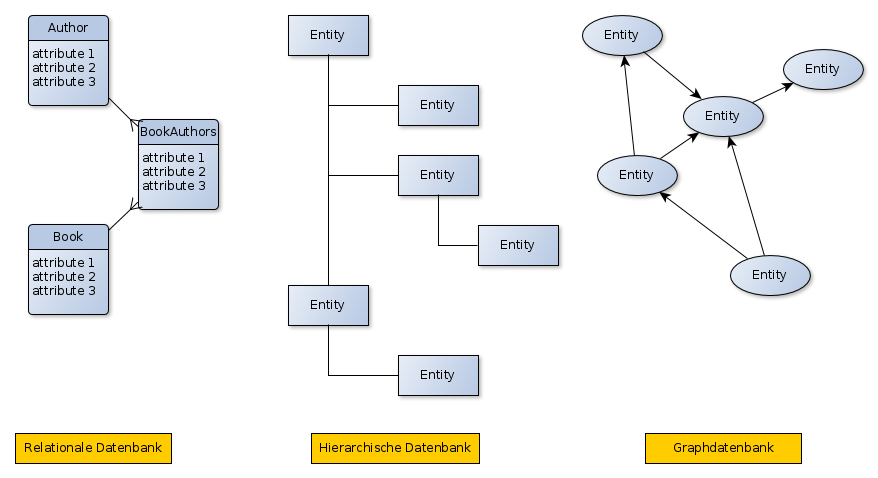
\includegraphics{bilder/datenbanktypen.png}}}
\caption{Darstellung der verschiedenen Datenbanktypen.\label{fig:datenbanktypen}\protect\footnotemark}
\end{figure}
\footnotetext{Eigene Darstellung mittels yEd}

\newpage

Gegeben seien die folgenden Aussagen über Hotels:
\lstset{caption={Aussagen über Hotels\protect\footnotemark},captionpos=b}
\begin{lstlisting}
    Ein Wellnesshotel ist ein Hotel.
    Ein Familienhotel ist ein Hotel.
    Wellnesshotels sind mit Familienhotels verwandt.
\end{lstlisting}

Verwendet man nun diese Aussagen über Hotels um daraus eine Graphdatenbank zu erstellen, so ergibt sich folgende Graphdatenbank:
\begin{figure}[htbp]
\centering \rotatebox{0}{\scalebox{0.5}[0.5]{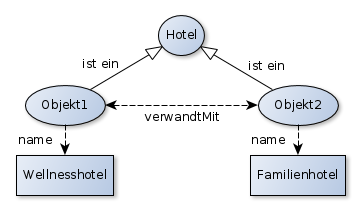
\includegraphics{bilder/hotels_graph.png}}}
\caption{Aussagen über Hotels als Graphdatenbank.\label{fig:hotels_graphdatenbank}\protect\footnotemark}
\end{figure}
\footnotetext{Eigene Darstellung mittels yEd}

In der Graphdatenbank existieren also zwei Objekte, \textit{``Objekt1''} und \textit{``Objekt2''}, mit den Eigenschaften \textit{``ist ein''}, \textit{``verwandtMit''} und \textit{``name''}.

Da eine Graphdatenbank eher eine hohe Abstraktionsebene darstellt, werden Wissensrepräsentationsformen sowie die Anwendung dieser im folgenden Kapitel ---~\ref{chap:wissensrepFormen}~\nameref{chap:wissensrepFormen}--- genauer erläutert.
